\documentclass[tikz, border=5pt]{standalone}
\usepackage{tikz}
\usepackage{amsmath}
\usepackage{xcolor}

% 需要的 TikZ 库
\usetikzlibrary{arrows.meta}
\usetikzlibrary{bending}
\usetikzlibrary{decorations.pathreplacing}
\usetikzlibrary{calc}

% 定义颜色
\definecolor{explanation-red}{RGB}{255,0,0}
\definecolor{explanation-blue}{RGB}{0,0,255}

% 定义分布曲线绘制命令
\newcommand{\gaussiancurve}[3]{
  % #1: x-offset, #2: scale factor, #3: label
  \begin{scope}[shift={(#1,0)}]
    \draw[thick] (-1.5,0) -- (1.5,0);
    \draw[thick] plot[domain=-1.5:1.5, samples=100] (\x, {#2*exp(-\x*\x/0.5)});
    \node[below, align=center, font=\small] at (0,-0.3) {#3};
  \end{scope}
}

\begin{document}
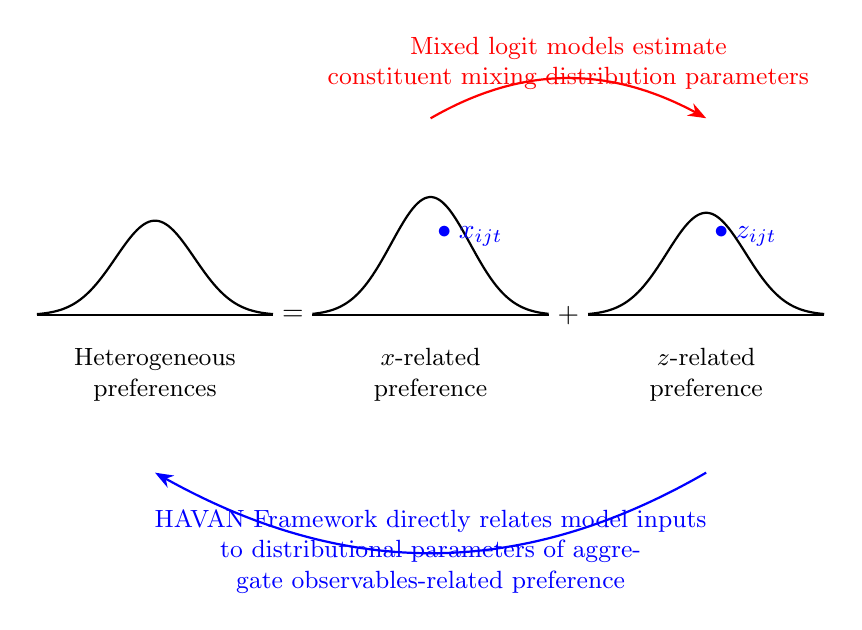
\begin{tikzpicture}[
  font=\sffamily,
  >={Stealth[bend]},
  node distance=2.5cm
]

% 三个分布曲线
\gaussiancurve{0}{1.2}{Heterogeneous\\preferences}
\gaussiancurve{3.5}{1.5}{$x$-related\\preference}
\gaussiancurve{7}{1.3}{$z$-related\\preference}

% 等式符号和点乘
\node at (1.75,0) {$=$};
\node at (5.25,0) {$+$};

% 变量标签
\node[explanation-blue] at (4,1) {$\bullet\; x_{ijt}$};
\node[explanation-blue] at (7.5,1) {$\bullet\; z_{ijt}$};

% 红色上方箭头和说明
\draw[->, explanation-red, thick, out=30, in=150] (3.5,2.5) to (7,2.5);
\node[explanation-red, align=center, font=\small] at (5.25,3.2) {Mixed logit models estimate\\constituent mixing distribution parameters};

% 蓝色下方箭头和说明
\draw[->, explanation-blue, thick, out=210, in=330] (7,-2) to (0,-2);
\node[explanation-blue, align=center, font=\small, text width=10cm] at (3.5,-3) {HAVAN Framework directly relates model inputs\\to distributional parameters of aggregate observables-related preference};

\end{tikzpicture}
\end{document}